\documentclass[assignment1.tex]{subfiles}
\begin{document}

\section*{3η Άσκηση}


\subsection*{Περιγραφή Προσομοίωσης}
Για την προσομοίωση του πειράματος μέτρησης της επιτάχυνσης της βαρύτητας εφαρμόστηκαν δύο μέθοδοι. Αρχικά ορίστηκε ένα διάνυσμα $\vec{L}$ με τα μήκη της εκφώνησης. Σε κάθε μήκος $L_i$, γίνεται προσομοίωση μέτρησης της περιόδου. 

Συγκεκριμένα, κάθε μέτρηση περιόδου, θεωρείται πως προκύπτει από την πραγματική περίοδο (\ref{eq:period}), για δοσμένη επιτάχυνση βαρύτητας \textlatin{g} (πχ $9.8\frac{m}{s^2}$) και μήκος εκκρεμούς $L_i$, στην οποία έχει προστεθεί ένας τυχαίος αριθμός. Δηλαδή η μέτρηση είναι μια τυχαία μεταβλητή $T_i = T + \delta T_i$, όπου $\delta T_i \sim N(0,1)\cdot \delta T$. Τελικά προκύπτει ένα νέο διάνυσμα $\vec{T}$.

\begin{equation}
T = 2\pi \sqrt{\frac{L}{g}}
\label{eq:period}
\end{equation}

Από κάθε ζεύγος τιμών $(L_i, T_i)$ υπολογίζεται έμμεσα η τιμή της επιτάχυνσης της βαρύτητας $g_i$ σύμφωνα με την εξίσωση (\ref{eq:g}), με σφάλμα που δίνεται από το νόμο διάδοσης σφαλμάτων (\ref{eq:gError}).

\begin{equation}
g_i = 4\pi^2 \frac{L_i}{T_i^2}, i=1,2,3,4
\label{eq:g}
\end{equation}

\begin{equation}
\delta g_i = 4\pi^2 \sqrt{\left(\frac{\delta L}{T_i^2}\right)^2 + \left(\frac{2L_i\delta T}{T_i^3}\right)^2}, i=1,2,3,4
\label{eq:gError}
\end{equation}

Η μέση τιμή των $g_i$ δίνει μια εκτίμηση για την επιτάχυνση της βαρύτητας $\bar{g}=\frac{1}{4}\sum_i g_i$, με σφάλμα $\delta g = \frac{1}{4}\sqrt{\sum_i \delta g_i^2}$.

Αν η εξίσωση (\ref{eq:period}) λυθεί ως προς $T^2$, τότε προκύπτει η εξίσωση (\ref{eq:linear}), η οποία είναι μια γραμμική συνάρτηση $T^2(L)$, με τη σταθερά $g$ κρυμμένη μέσα στο συντελεστή διεύθυνσης της ευθείας. 

\begin{equation}
T^2 = \frac{4\pi^2}{g}L
\label{eq:linear}
\end{equation}

Τα ζεύγη $(L_i, T_i^2)$ μπορούν να χρησιμοποιηθούν για να χαραχτεί μια ευθεία ελαχίστων τετραγώνων, η οποία θα είναι κοντά στην εξίσωση (\ref{eq:linear}). Από την κλίση της ευθείας ελαχίστων τετραγώνων υπολογίζεται η επιτάχυνση της βαρύτητας σύμφωνα με την εξίσωση (\ref{eq:gLS}).

\begin{equation}
g = \frac{4\pi^2}{A}
\label{eq:gLS}
\end{equation}

Ο αλγόριθμος ευθείας ελαχίστων τετραγώνων δίνει το σφάλμα της κλίσης $\delta A$, αλλά αυτό δεν συμπίπτει με το σφάλμα $\delta g$. Για τον προσδιορισμό του $\delta g$ απαιτείται εφαρμογή του νόμου διάδοσης σφαλμάτων στην εξίσωση(\ref{eq:gLS}), δηλαδή η εξίσωση (\ref{eq:gErrorLS}).

\begin{equation}
\delta g = \frac{4\pi^2}{A^2}\delta A
\label{eq:gErrorLS}
\end{equation}

To πείραμα προσομοιώνεται δύο φορές, όμως στη δεύτερη εκτέλεση υπάρχει ένα σταθερό συστηματικό σφάλμα στη μέτρηση του μήκους του εκκρεμούς, $\delta L_{sys}=0.05m$. Για καλύτερη σύγκριση των δύο μεθόδων, δεν επαναλαμβάνονται η μετρήσεις της περιόδου.

Αναμένεται η ευθεία ελαχίστων τετραγώνων να είναι μετατοπισμένη κατά $0.05m$ δεξιά.

\subsection*{Αποτελέσματα Προσομοίωσης}

Τα αποτελέσματα της προσομοίωσης είναι συγκεντρωμένα στον Πίνακα \ref{table:results}. Η θεωρητική τιμή της επιτάχυνσης της βαρύτητας είχε τεθεί ως $9.8\frac{m}{s^2}$ αλλά παρατηρείται ότι και οι δύο μέθοδοι έχουν σημαντική απόκλιση της τάξης του $10\%$. Η απόκλιση μπορεί να δικαιολογηθεί από το σφάλμα μέτρησης του χρόνου της περιόδου που κυμαίνεται από $5\%$ - $13\%$.

Στο πρώτο πείραμα και οι δύο μέθοδοι βρίσκουν περίπου την ίδια τιμή για την επιτάχυνση της βαρύτητας αλλά το σφάλμα της μεθόδου ελαχίστων τετραγώνων είναι μεγαλύτερο από αυτό της μέσης τιμής. Αυτή η κακή επίδοσης της μεθόδου ελαχίστων τετραγώνων, οφείλεται στην χρήση του κανόνα διάδοσης σφαλμάτων (\ref{eq:gErrorLS}).

\begin{table}[ht]
\centering
\begin{tabular}{||c c c||} 
 \hline
 $\delta L_{syst}$& Μέση Τιμή & Ελάχιστα Τετράγωνα \\ [0.5ex] 
 \hline\hline
 0 & $10.4\pm 0.9$ & $10.2 \pm 1.9$ \\ 
 0.05 & $11.8\pm 1.1$ & $10.2 \pm 1.9$ \\ [1ex] 
 \hline
\end{tabular}
\caption{Αποτελέσματα Προσομοίωσης}
\label{table:results}
\end{table}

Ωστόσο, μολονότι η μέθοδος ελαχίστων τετραγώνων έχει μεγαλύτερη ανακρίβεια, υπερτερεί της μέσης τιμής γιατί είναι αναίσθητη σε συστηματικά σφάλματα. Όπως φαίνεται από το Σχήμα \ref{fig:least_squares}, αλλά και τις μετρήσεις του Πίνακα \ref{table:results}, το συστηματικό σφάλμα δεν μετέβαλλε την τιμή του στατιστικού σφάλματος της ευθείας ελαχίστων τετραγώνων.

\begin{figure}[hp]
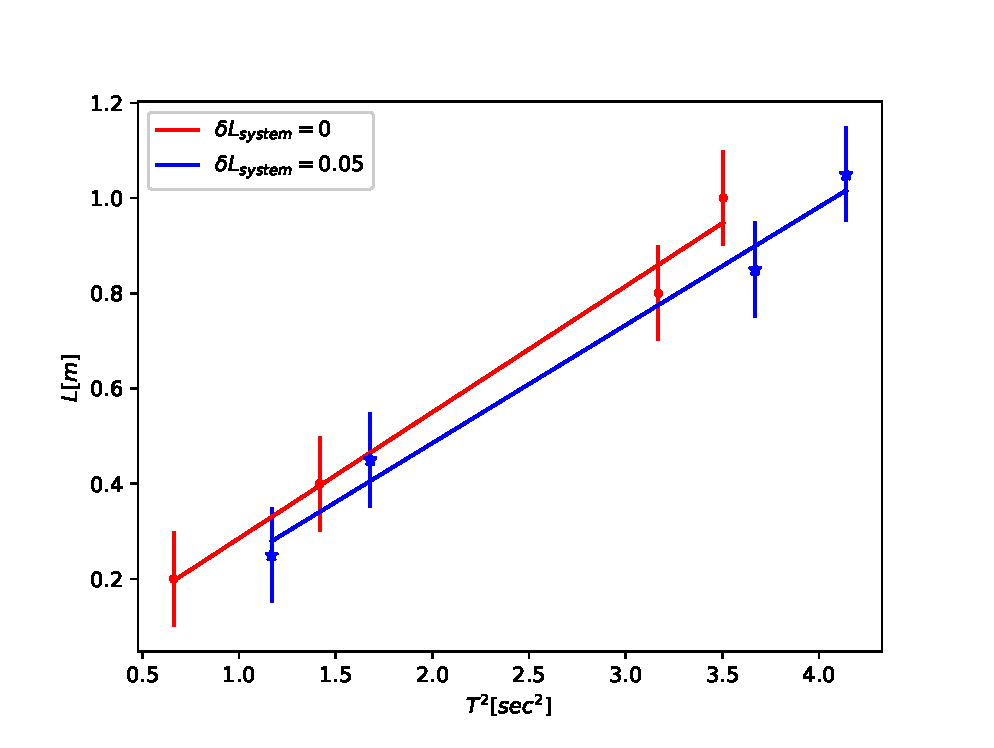
\includegraphics[width=0.9\textwidth]{experiment.eps}
\centering
\caption{Ελάχιστα Τετράγωνα Προσομοίωσης}
\label{fig:least_squares}
\end{figure} 

\FloatBarrier

\subsection*{Πηγαίος Κώδικας}

Παρακάτω ακολουθεί ο κώδικας που γράφτηκε σε \textlatin{Python} και έγινε χρήση της βιβλιοθήκης \textlatin{Numpy}.

\selectlanguage{english}
\lstinputlisting[style=python, firstline=8]{mc_experiment.py}

\end{document}